\documentclass[11pt]{article}
\usepackage[utf8]{inputenc} % Para caracteres en espa�ol
\usepackage{amsmath,amsthm,amsfonts,amssymb,amscd}
\usepackage{multirow,booktabs}
\usepackage[table]{xcolor}
\usepackage{fullpage}
\usepackage{lastpage}
\usepackage{enumitem}
\usepackage{floatrow}
\usepackage{multicol}
\usepackage{fancyhdr}
\usepackage{mathrsfs}
\usepackage{wrapfig}
\usepackage[final]{pdfpages}
\usepackage{setspace}
\usepackage{esvect}
\usepackage{calc}
\usepackage{multicol}
\usepackage{cancel}
\usepackage{graphicx}
\graphicspath{ {picturesB/} }
\usepackage[retainorgcmds]{IEEEtrantools}
\usepackage[margin=3cm]{geometry}
\usepackage{amsmath}
\newlength{\tabcont}
\setlength{\parindent}{0.0in}
\setlength{\parskip}{0.05in}
\usepackage{empheq}
\usepackage{framed}
%\usepackage{newtxmath}
\usepackage{euscript}
\DeclareMathAlphabet{\mathpzc}{T1}{pzc}{m}{it}
\usepackage[most]{tcolorbox}
\usepackage{xcolor}
\colorlet{shadecolor}{orange!15}
\parindent 0in
\parskip 12pt
\geometry{margin=1in, headsep=0.25in}
\theoremstyle{definition}
\newtheorem{defn}{Definition}
\newtheorem{reg}{Rule}
\newtheorem{exer}{Exercise}
\newtheorem{note}{Note}
\newcommand{\volume}{{\ooalign{\hfil$V$\hfil\cr\kern0.08em--\hfil\cr}}}
\newcommand{\parr}{\mathbin{\|}} % Parralel Symbol
\begin{document}
\setcounter{section}{1}%Section we want -1
\setcounter{page}{24} %Page we want
\setcounter{equation}{35}%Equation we want -1
\def\thepart{\arabic{part}}
\setcounter{part}{9}
\numberwithin{equation}{part}

 \pagestyle{fancy}
\fancyhf{}
\rhead{Section 9:  Electrostatic Propulsion - Hall-Effect Thrusters}
\rfoot{Page \thepage}
\thispagestyle{empty}

\begin{center}
{\LARGE \bf Section 9:  Electrostatic Propulsion}\\
{\large AE435}\\
Spring 2018
\end{center}
\vspace{5mm}
\section{Hall-Effect Thrusters}
\vspace{25mm}
\tableofcontents
\newpage
Hall thrusters have a cylindrical channel with an interior anode, a magnetic circuit that produces a primarily radial magnetic field across the channel, and a cathode external to the channel.   The details of the channel structure and magnetic field shape determine the performance, efficiency, and lifetime. Anode efficiency 50-60$\%$, specific impulse is around 1000-2000sec but at lower specific impulse has higher thrust at the same power. 

Efficiency and specific impulse are typically lower than ion thrusters, the thrust-to-power ratio is higher and Hall thruster requires fewer power supplies to operate.
 
There are two main types of Hall thrusters:
\begin{enumerate}
\item Hall-effect thruster (HET, a.k.a., Hall thruster, stationary plasma thruster (SPT), magnetic layer thruster are all the same thing)  These devices have a dielectric insulating wall in the plasma channel.  It is typically boron nitride (ceramic insulator).  Ideal because of its low sputtering yield and relatively low secondary electron emission coefficient.
\item Thruster with anode layer (TAL)  Dielectric channel wall is replaced with metallic conducting wall.  Considerably shorter geometry, with strong electric field close to the anode. 
 \end{enumerate}

 \begin{center}
{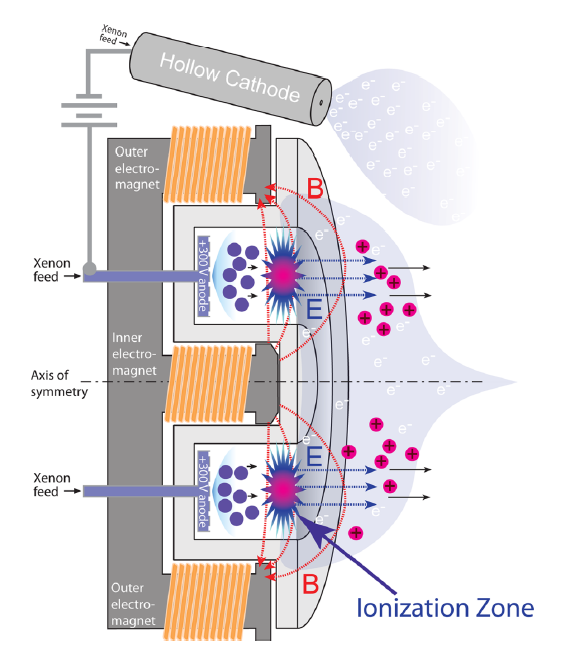
\includegraphics[scale=0.55]{15.png}}
\end{center}

HET is dominant in U.S.  TAL was developed by Russians in 1960s, not as much research focus anymore.  HET tends to have better efficiency and performance due to longer channel for increased ionization path length and lower electron transport.
\begin{center}
{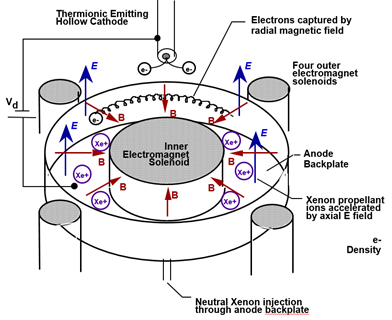
\includegraphics[scale=1.6]{16.png}}
\end{center}
 \begin{center}
{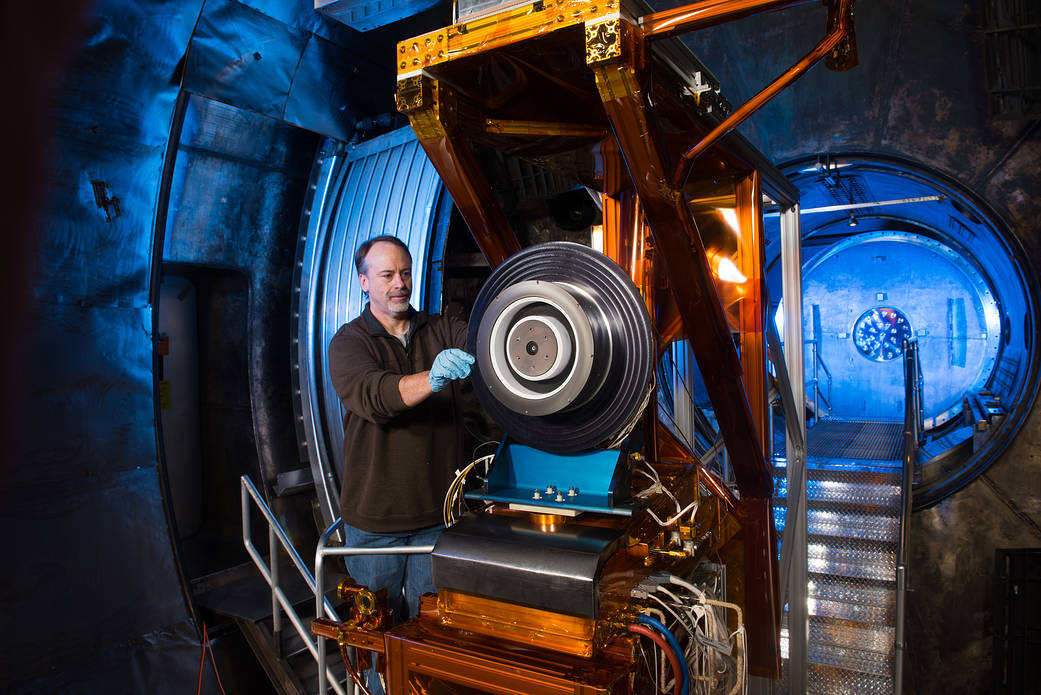
\includegraphics[scale=1.5]{17.jpg}}
\end{center}
12.5kW HERMeS Hall thruster
 \begin{center}
{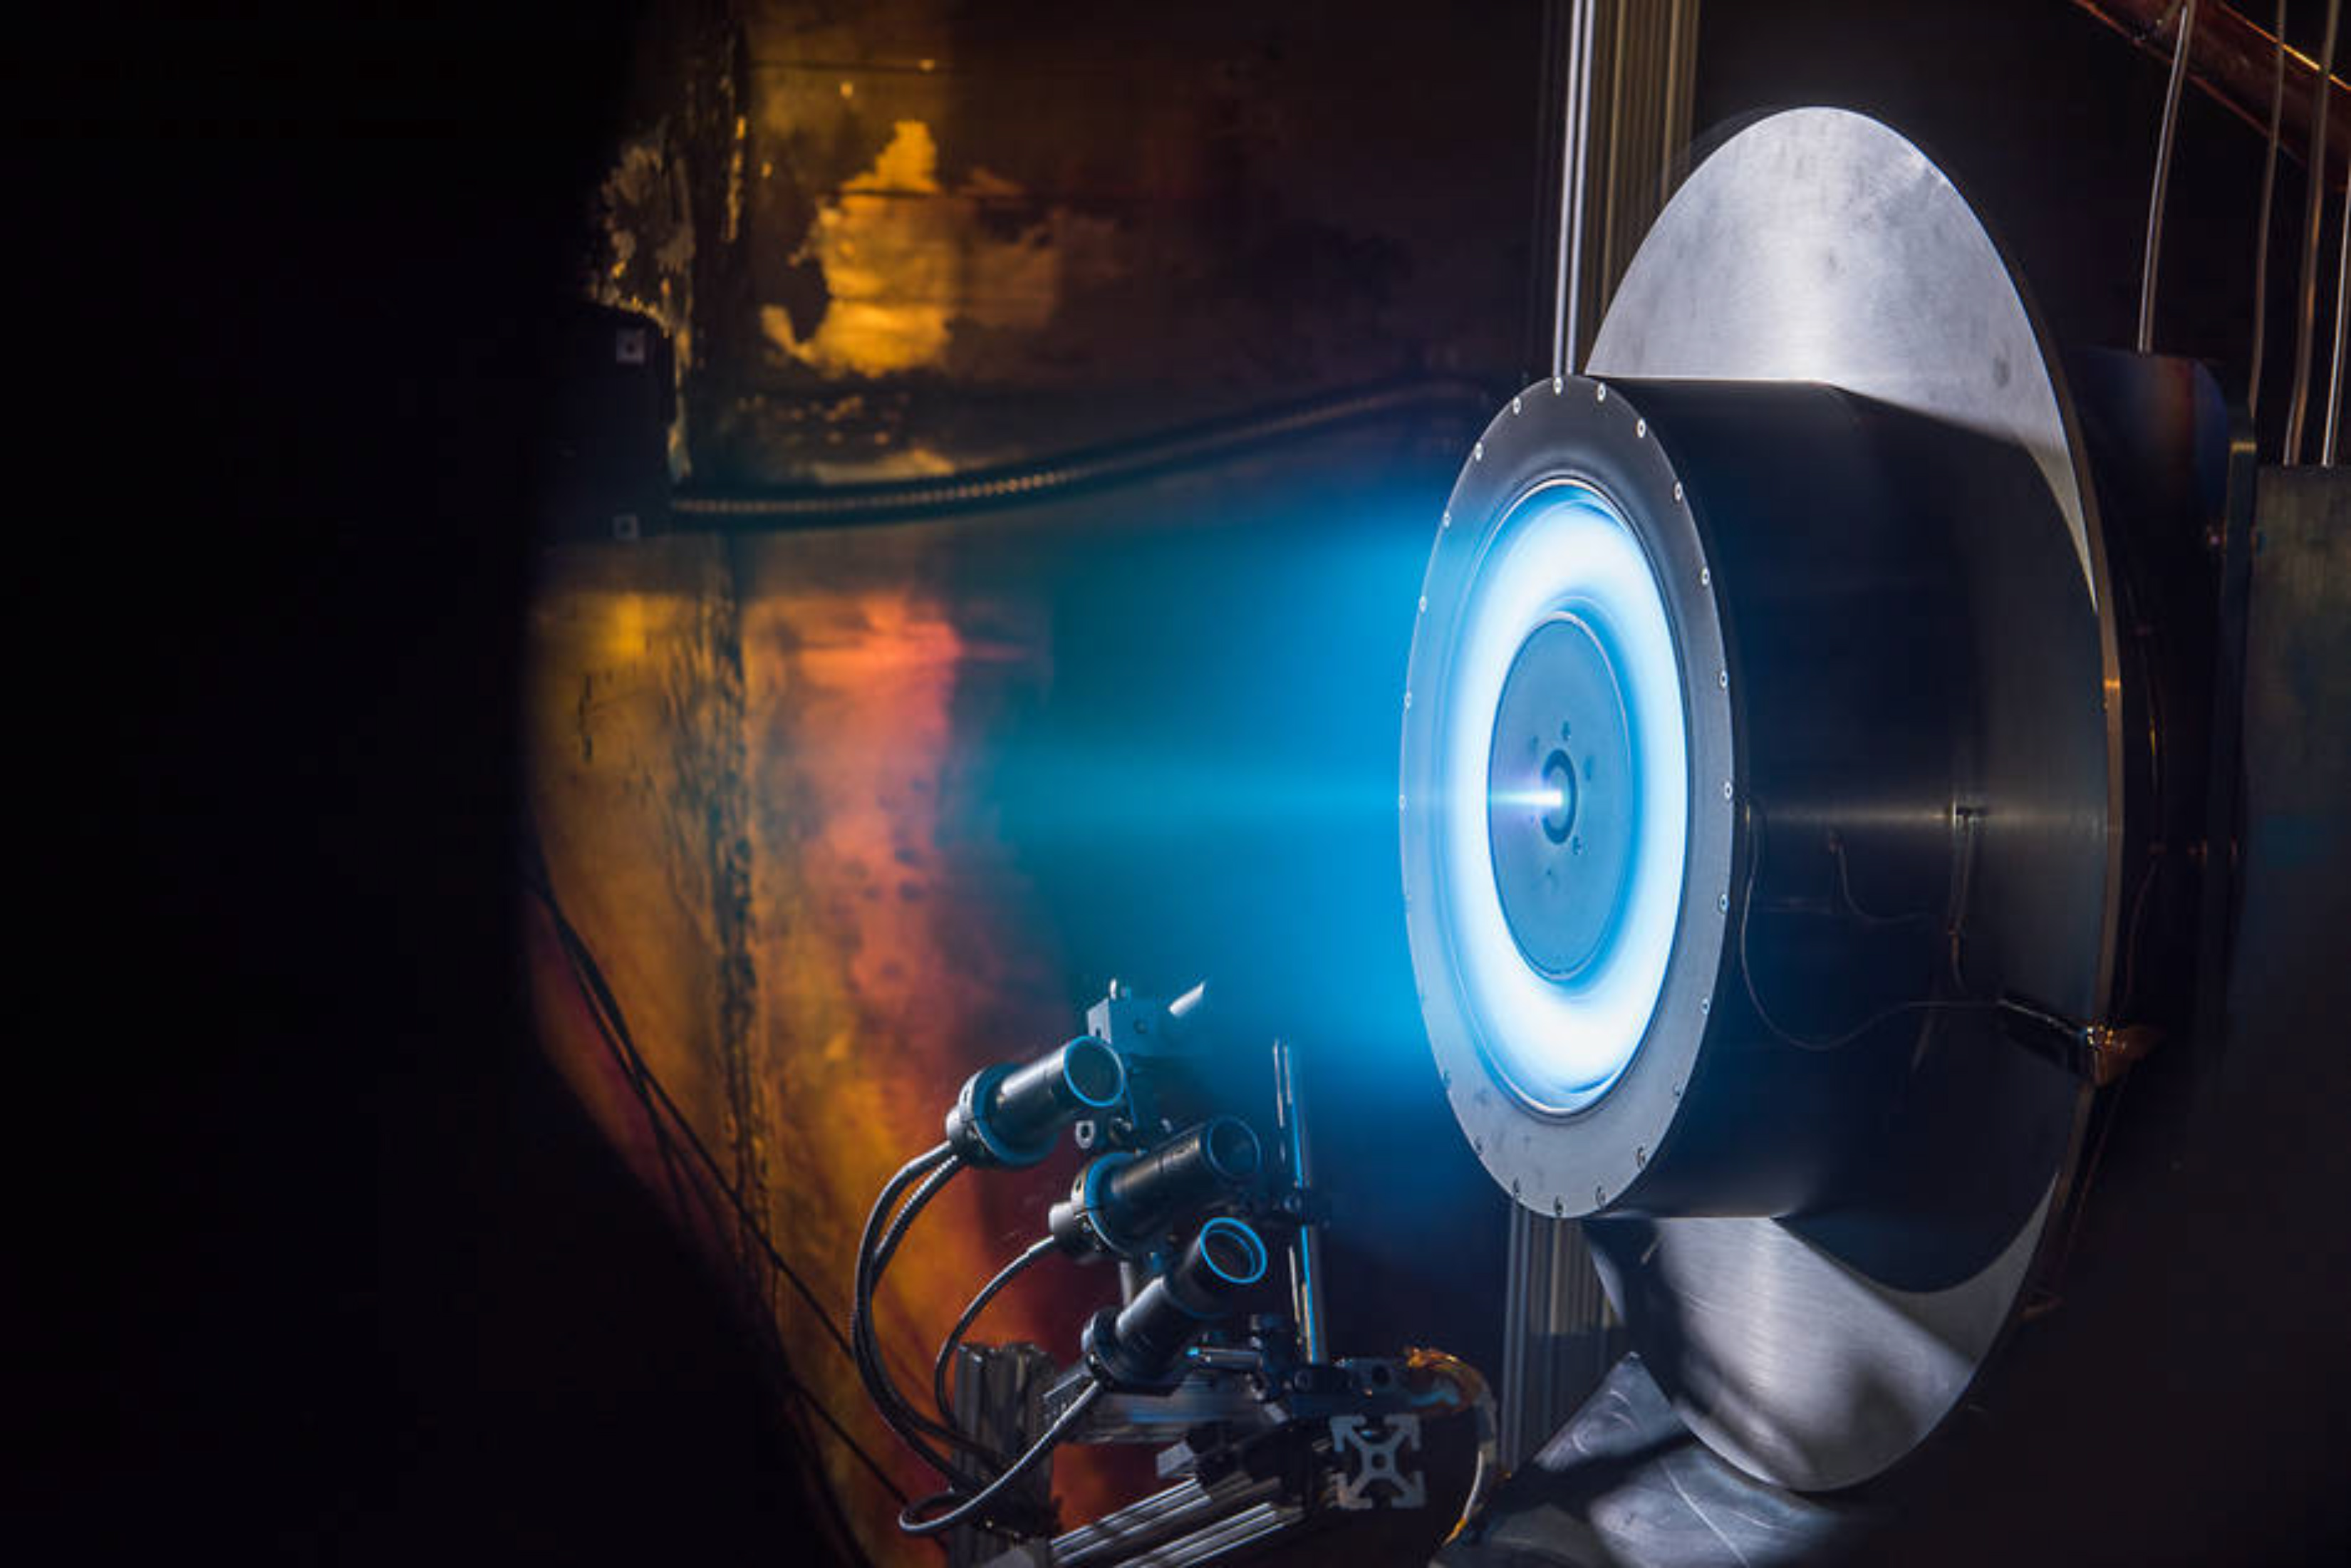
\includegraphics[scale=0.5]{18.jpg}}
\end{center}
 \newpage
PPS-1350 SNECMA
 \begin{center}
{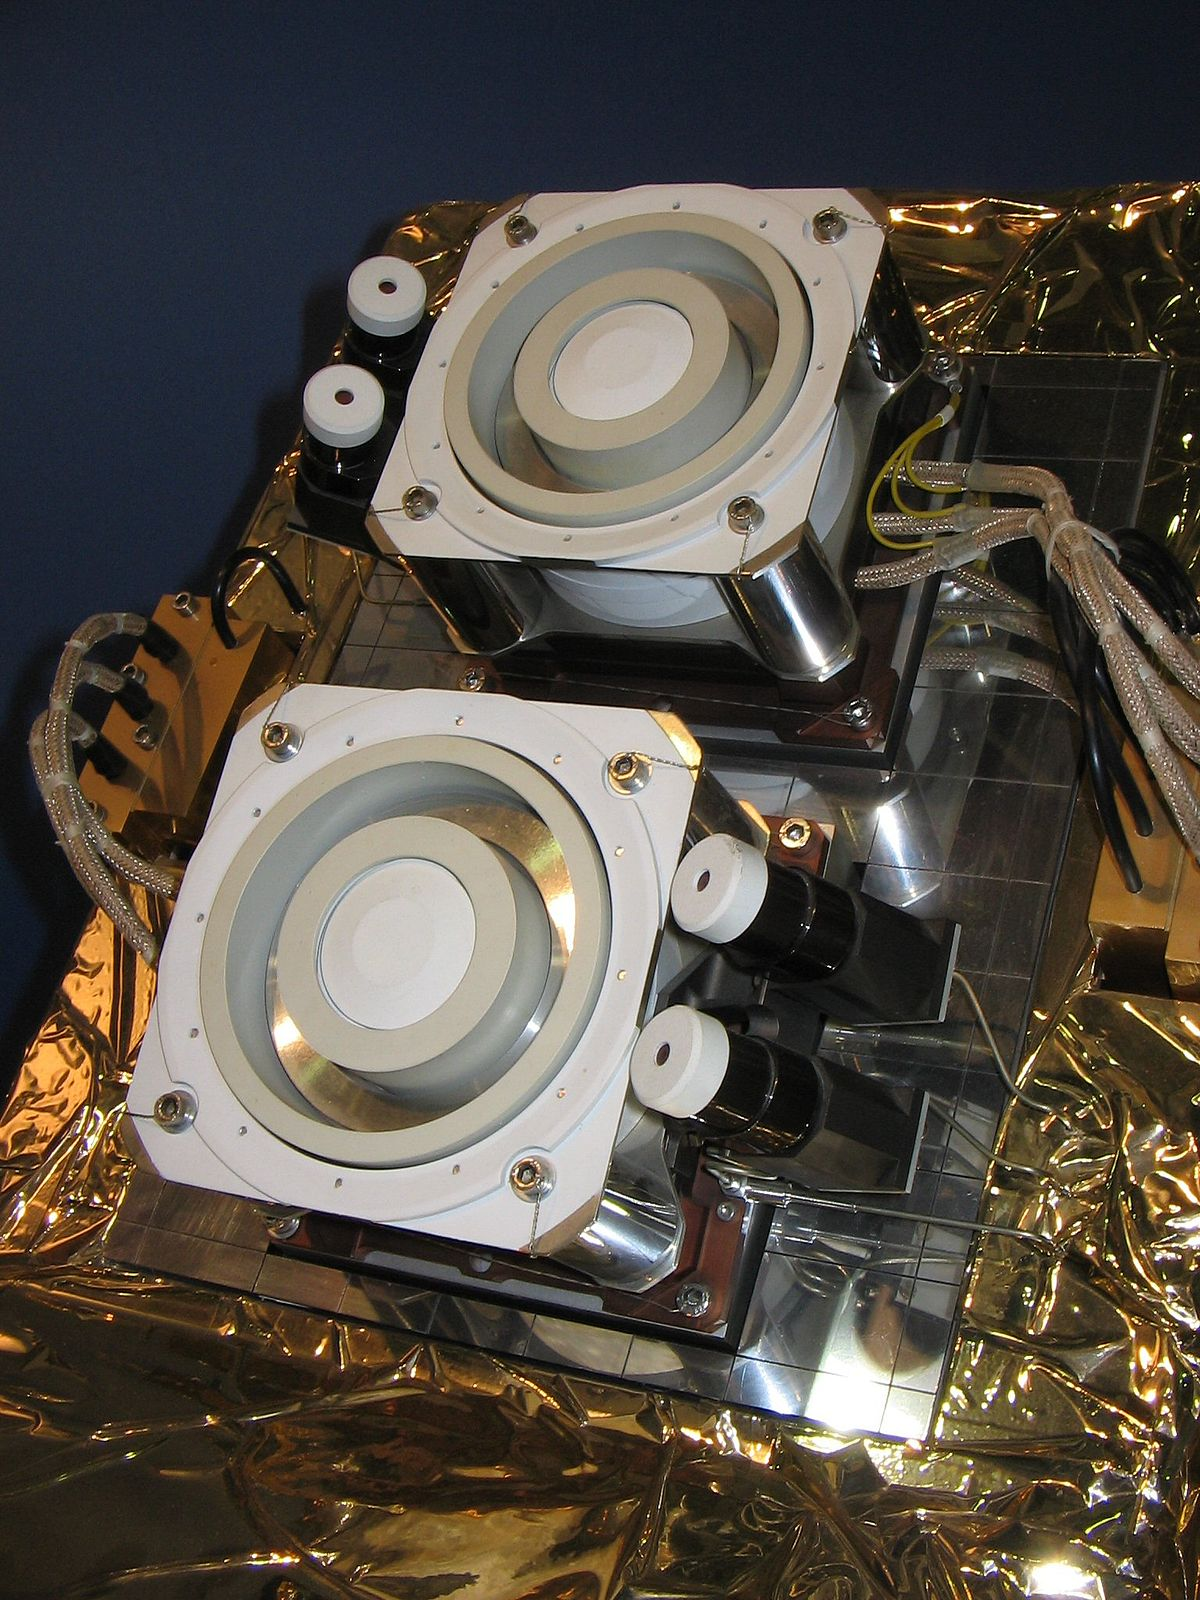
\includegraphics[scale=0.5]{19.jpg}}
\end{center}
 
Aerojet XR-5
\begin{center}
{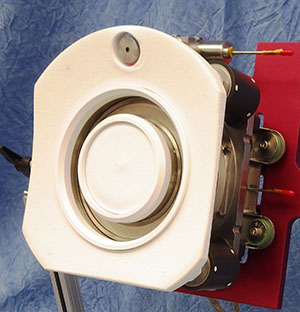
\includegraphics[scale=0.5]{20.jpg}}
\end{center}

 \newpage
\subsection{Operation and Scaling}
Propellant injected at the anode expands toward the exit plane and encounters the plasma generated in the channel.  This crossed field discharge extends over a length scale, L, and produces a significant plasma density of characteristic width, w, which is basically the channel width.  This plasma region is symmetric about the cylindrical channel and has a symmetric area $A_e$.  Applied magnetic field is primarily vertical (radial) in this intense plasma region.%
 
 %Magnetic field is having a significant effect on thier motion.
In Hall thruster the electrons are magnetized and forced to execute ExB drift in the azimuthal direction.  Therefore we require the electron Larmor radius to be much smaller than the characteristic size of the plasma length scale, L, that is:
 \begin{equation}
 \begin{aligned}
 r_{L,e} = \frac{V_{th}}{\omega_B} = \frac{m}{e \, B} \sqrt{\frac{8 \, k \, T_e}{\pi \, m}} \ll L
 \end{aligned}
 \end{equation}
 
And the electron Hall parameter must be much greater than 1.
 
  \begin{equation}
 \begin{aligned}
 \Omega_e^2 = \frac{\omega_B^2}{\nu^2} \gg 1
 \end{aligned}
 \end{equation}
 Where
   \begin{equation*}
 \begin{aligned}
\nu &=\text{Total collision frequency of electrons}\\
\omega_B &=\text{Cyclotron frequency of electrons}
 \end{aligned}
 \end{equation*}
 


We saw that a large value of the Hall parameter reduces the cross-field electron mobility in (III. B. 2.).
 
Similarly, we require the ions to NOT be magnetized, that is, the ion Larmor radius is much larger than the characteristic size, L. We want the ions to just shoot straight out so we don't want them experience an ExB drift.
 
  \begin{equation}
 \begin{aligned}
  r_{L,i} = \frac{V_{i}}{\omega_B} = \frac{M}{e \, B} \sqrt{\frac{2 \,e \, V_b}{M}} \gg L
 \end{aligned}
 \end{equation}
 
where beam voltage, $V_b$, the total potential drop that is accelerating the ions.
 \newpage
The magnetic field have a typical axial profile as shown below.  $dB/dz > 0$ critical for stability!
\begin{center}
{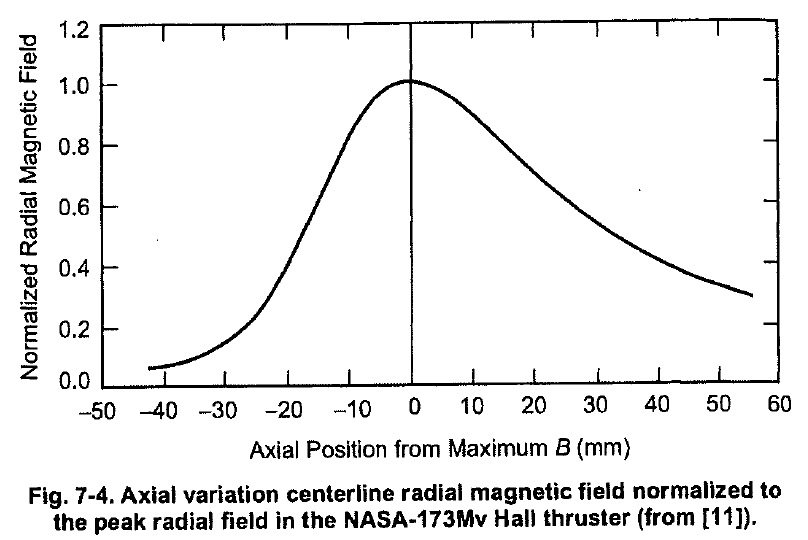
\includegraphics[scale=0.65]{21.png}}
\end{center}
\begin{center}
{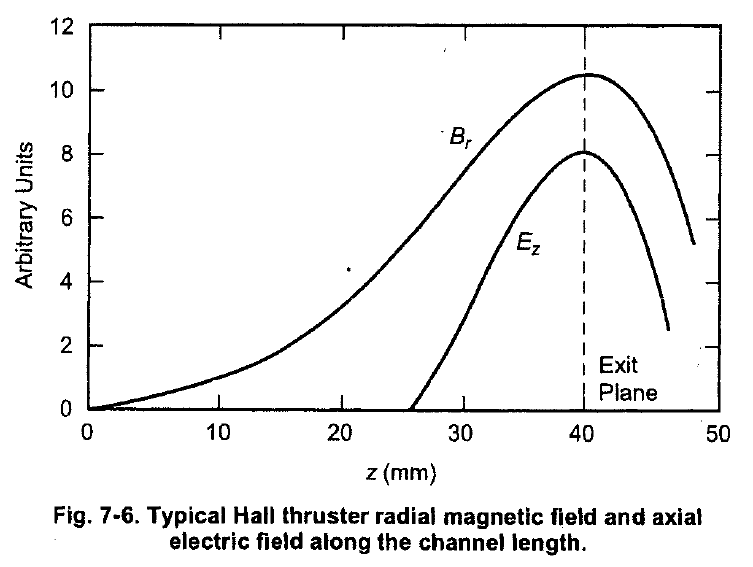
\includegraphics[scale=0.65]{22.png}}
\end{center}
Notice dB/dz is greater than 1 so the 0 location is the exit plane, everything to the left is inside the discharge chamber, and everything to the right is outside the discharge chamber. 
 
What if we had a negative dB/dz? We would have another trapping region within the channel which is not desired.
 
The region of high magnetic field is at the exit plane (peak field ~150-200 G), and is where the electrons are confined and therefore where the largest potential drop occurs (and therefore largest electric field, ).  Ions are accelerated by this electric field and this region is called the "acceleration region".  The "ionization" region precedes it, but the two overlap to give rise to a spread in the beam energy (unlike ion thruster which has distinct/separated plasma creation and acceleration regions).


 \subsubsection{Hall Curent Scaling}
\begin{center}
{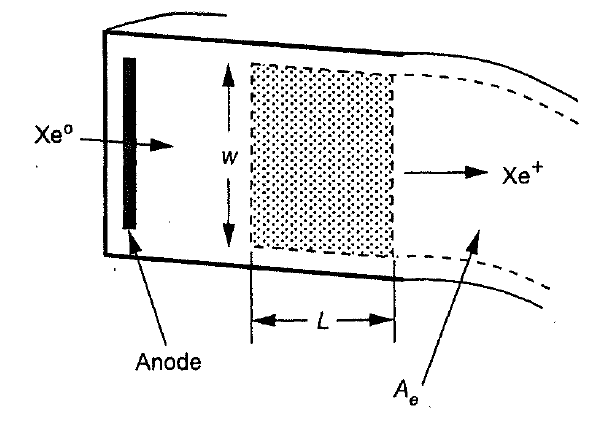
\includegraphics[scale=0.65]{23.png}}
\end{center}
In the strong $B_r$ and $E_z$ region, electrons move in Hall current in azimuthal direction.  That is, they ExB drift, with velocity given by (3.17):
  \begin{equation}
 \begin{aligned}
 |v_{_{E\times B}}| = \frac{E_z}{B_r}
 \end{aligned}
 \end{equation}
 The hall current is then:
 \begin{shaded}
 \textbf{Hall Current:}
  \begin{equation}
 \begin{aligned}
 I_H \cong n_e \, e  \, \omega \, \frac{V_d}{B}
 \end{aligned}
 \end{equation}
where
  \begin{equation*}
 \begin{aligned}
\omega &= \text{Plasma height or channel height}\\
V_d \approx V_b &= \text{Discharge voltage, which is also approximately beam voltage }\\
\end{aligned}
 \end{equation*}
\end{shaded}
\newpage
Hall current is approximately constant for given plasma density or beam current, and is proportional to the discharge voltage.  Since the ion current leaving the plasma to form the beam is:
 
 %Increase the magneitci field, the current decreases. 
 
  \begin{equation}
 \begin{aligned}
 I_i = n_i \, e \, v_i \, A_e \cong n_i \, e \, \sqrt{\frac{2 \, e \, V_d}{M}} \, 2 \, \pi \, R \, \omega
 \end{aligned}
 \end{equation}
where
  \begin{equation*}
 \begin{aligned}
R &= \text{Average Radius of the Plasma Channel} \\
2 \, \pi \, R \, \omega &\sim A_e
 \end{aligned}
 \end{equation*}
 
Then, using (9.41) in (9.40), the hall current becomes:
 
  \begin{equation}
 \begin{aligned}
 I_H \cong \frac{I_i}{2 \, \pi \, R \, B} \, \sqrt{\frac{M \, V_d}{2 \, e}}
 \end{aligned}
 \end{equation}
 
Increasing beam current will increase the circulating Hall current for a given magnetic field and discharge voltage.
We also see increasing magnetic field will decreases the hall current. We will see hall currents range from 10's-100's of Amps. Ion currents are around 1-10's of amps. 
 \newpage
\subsubsection{Ionization Length and Scaling}
When we put in the neutrals, we want to ionize all of the nuetrals. We will find a length scale that allows us to have ionization for different characteristics. In other words, neutrals enter the "ionization" region and become ionized.  A flux of neutrals enters the "ionization" region and this flux will decrease with distance into the region as neutrals become ionized.  To ionize most/all of the neutrals, the plasma must have some thickness, L, which we can estimate here. 
 
The rate of change of neutral atoms due to ionization is:
  \begin{equation}
 \begin{aligned}
 \frac{\mathrm{d} n_n}{\mathrm{d} t} = -n_n \, n_e \, <\sigma_i \, v_e>
 \end{aligned}
 \end{equation}%Decreasing with time becuase the amount of neturals to ionize is decreasing as we ionize more and more.
 
where we define the flux as: %Number per second per unit area. 
  \begin{equation}
 \begin{aligned}
 \Gamma_n = n_n \, v_n
 \end{aligned}
 \end{equation}
 
Equation 9.43 then becomes: 
 
  \begin{equation*}
 \begin{aligned}
 \frac{\mathrm{d} \Gamma}{\mathrm{d} t} = \frac{\mathrm{d} n}{\mathrm{d} t}\frac{\mathrm{d} z}{\mathrm{d} t} + n_n \, \frac{\mathrm{d}^2 z}{\mathrm{d} t^2}
 \end{aligned}
 \end{equation*}
 Where
   \begin{equation*}
 \begin{aligned}
\frac{\mathrm{d} z}{\mathrm{d} t} & = v_n & \qquad &\text{Neutral Velocity}\\
n_n \, \frac{\mathrm{d}^2 z}{\mathrm{d} t^2} &= 0 & \qquad &\text{No Neutral Acceleration}
 \end{aligned}
 \end{equation*}
 Such that...
  \begin{equation}
 \begin{aligned}
 \frac{\mathrm{d} \Gamma}{\mathrm{d} t} = \frac{-n_n \, n_e \, <\sigma_i \, v_e>}{n_n \, v_n}\,\mathrm{d}z = \frac{-n_e \, <\sigma_i \, v_e>}{v_n}\,\mathrm{d}z
 \end{aligned}
 \end{equation}
 
which has solution:
  \begin{equation}
 \begin{aligned}
 \Gamma_n(z) = \Gamma(0)\exp(\frac{-z}{\lambda_i})
 \end{aligned}
 \end{equation}
where $\Gamma(0)$ is $\Gamma$ at $z = 0$.

And the ionization mean free path is:
 \begin{shaded}
 \textbf{Ionization Mean Free Path}
  \begin{equation}
 \begin{aligned}
 \lambda_i = \frac{v_n}{n_e <\sigma_i \, v_e>}
 \end{aligned}
 \end{equation}%average distance a neutral particle must travel before it becomes ionized
 \end{shaded}
 
The fraction of neutrals that are ionized after traversing a plasma of length L is:
 %In other words, the flux (ionized neutrals) coming out over the flux (neutrals) coming in
  \begin{equation}
 \begin{aligned}
 \frac{\Gamma_{\text{exit}}}{\Gamma_{\text{incident}}} = 1 - \exp\bigg(\frac{-L}{\lambda_i}\bigg)
 \end{aligned}
 \end{equation}%How the flux changes as the numver of neutrals moves through the plasma.
 
For example, to have 95$\%$ ionized, then the length scale we seek is:
 
  \begin{equation}
 \begin{aligned}
 L = -\lambda_i \, \ln(1-0.95) = 2.996 \, \lambda_i \cong \frac{3 \, v_n}{n_e <\sigma_i \, v_e>}
 \end{aligned}
 \end{equation}
 
or, the plasma thickness $(L)$ must be at least 3 times the ionization mean-free path.  But some ions will hit the channel walls and re-enter the plasma as neutrals, so the plasma thickness, $L$ , should significantly exceed the ionization mean free path, that is:
 
  \begin{equation}
 \begin{aligned}
 \frac{\lambda_i}{L} \ll 1
 \end{aligned}
 \end{equation}
 
Tradeoff: Length-scale long enough to ionize the propellant but not long enough where we deposit a lot of our energy to the channel walls. 
 
Notice in 9.49 how L changes for $v_n$, where $v_n$ is the neutral velocity. Lets say we go from xenon neutrals to krypton or argon neutrals.What happens to $v_n$, they will decrease. Temperature of neutrals coming into chamber are coming through the anode will be around 500Cish, much lower than electron temperature. If the mass of the propellant decreases, the neutral velocity increases , therefor the length scale will need to be longer assuming the same ionization rate. 

Clearly, higher ionization rate leads to a shorter ionization thickness, we don't need it to be that long if we can ionize much quicker. 
 
From our example above, this ratio should be $< 1/3 = 0.33$.
 
Actual channel length is L (plasma thickness), plus the length required to demagnetize the plasma at the anode.  Needs to be long enough so that the Bfield decreases at the anode and particles not magnetized at the anode.  This axial magnetic field gradient of the radial magnetic field is critical for thruster performance, and results in higher thruster efficiency, $\frac{\partial B}{\partial z} > 0$.
 
Want almost zero field at the anode (helps maintain plasma at the anode potential, reduces sheath potential drop), but want strong radial field at exit.  Additionally, magnetic field profile at the thruster exit strongly affects closed electron drifts in azimuthal direction AND has ability to focus ions in axial direction AND can reduce ion bombardment of the walls, improving ion trajectories. 
\begin{center}
 \begin{table}[H]
 \centering
 \begin{tabular}{|c|l|r|r|}
  \hline
 && \\&&\\ &&\\ && \\
 \parbox[t]{2mm}{\multirow{1}{*}{\rotatebox[origin=c]{90}{Standard Model}}} & \hspace{80mm} &  \hspace{70mm} \\&& \\&&\\ && \\&&\\ && \\&&\\&&\\&&\\ && \\
 \hline
  \hline
 && \\&&\\ &&\\ && \\
 \parbox[t]{2mm}{\multirow{1}{*}{\rotatebox[origin=c]{90}{Ion Focusing Bfield}}} & \hspace{80mm} &  \hspace{70mm} \\&& \\&&\\ && \\&&\\ && \\&&\\&&\\&&\\ && \\
 \hline
   \hline
 && \\&&\\ &&\\ && \\&&\\&&\\&&\\
 \parbox[t]{2mm}{\multirow{1}{*}{\rotatebox[origin=c]{90}{Magnetic Shielding}}} & \hspace{80mm} &  \hspace{70mm} \\&& \\&&\\ && \\&&\\ && \\&&\\&&\\&&\\ && \\&&\\&&\\
 \hline
 \end{tabular}
 \end{table}%how to shape the magnetic fieed to shield the deilectricc disharge chamber and prevent cosine loss...
\end{center}

%Last couple of scaling relationships are...
Additionally, properly designed HET ionizes almost all propellant, such that:
 
The rate at which neutrals are being converted into ions is equal to the rate at which neutrals are incident on the plasma. 
 \begin{equation}
 \begin{aligned}
 n_e \, n_n \, <\sigma_i \, v_e> \, A_e \, L \approx n_n \, v_n \, A_e
 \end{aligned}
 \end{equation}
 This relationship is what gave us L above, but we will relate it to the hall current.
 
Then with (9.42) Hall current:

  \begin{equation}
 \begin{aligned}
 L = \frac{v_n}{n_e \, <\sigma_i \, v_e>} = \frac{v_n \, e \, w \, V_d}{I_H \, B \, <\sigma_i \, v_e>}
 \end{aligned}
 \end{equation}
 %This lengthscale 
Ionization region length must increase with neutral gas velocity, and can decrease with ionization rate coefficient.
 
If the neutrals are coming in with faster velocity(Smaller lighter propellant xenon to argon) we need a longer length-scale to get that ionized. IF we can ionize faster, we don't need as long of a length scale because we are ionizing faster.
 
Additional scaling laws for optimized Hall thrusters are:
 
  \begin{equation}
 \begin{aligned}%Power proprto thrust proptu outside radius of the thruster. If we want more thrust we must increase the overall size. .... Curernt propto outerdiameter squared therefore current density is a constant for a ghall thruster..... w (channel width)
 \text{power} &\propto \text{thrust} \propto R^2 \\ \\
 I_d &\propto R^2 \quad \rightarrow \quad j \propto \frac{I_d}{R^2} = const\\ \\
 \dot{m} &\propto R^2 \\ \\
 \omega &= R(1 - const) \\ \\ 
 A_e &= \pi(R^2 - r^2)
 \end{aligned}
 \end{equation}
 
 
 
where R is outside radius of the channel.  Optimum current density is essentially constant as the thruster size changes.  Typical current density is 0.1 to 0.15 A/cm2.  At given discharge voltage, power density in a Hall thruster is also constant.  Higher power density requires increasing voltage.

Remember that power is basically the discharge voltage times the discharge current which is proportional to...

 \begin{equation*}
 \begin{aligned}
 P = V_d \, I_d \propto V_d \, j \, R^2
 \end{aligned}
 \end{equation*}
 
 \newpage
For a given discharge voltage, current density is a constant, power density will be constant as well. If we want to increase it we must increase Voltage discharge.

  \begin{equation*}
 \begin{aligned}
 \frac{P}{R^2} \propto V_d \, j
 \end{aligned}
 \end{equation*}
 
 \begin{center}
{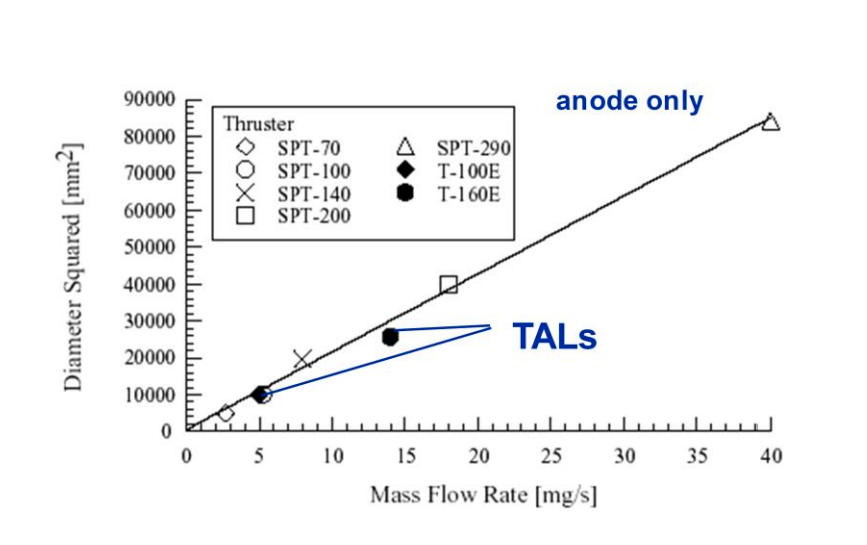
\includegraphics[scale=0.4]{24.png}}
\end{center}
 
\underline{Xenon Rule of 10's}

For xenon, 1 A of thruster current requires approximately 1 mg/s of propellant (mass flow rate) , which is approximately 10 sccm (standard cubic centimeters per minute) of volumetric flow rate
 
\underline{Magnetic Shielding} 

Recently magnetic shielding has been developed to keep ions from accelerating into and bombarding the channel walls.  Significantly increases lifetime (almost infinite lifetime).
 
 \begin{center}
{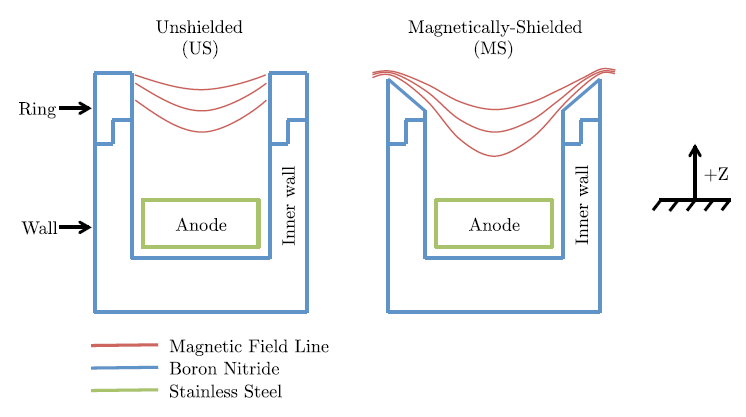
\includegraphics[scale=0.5]{25a.png}}
\end{center}
 
%Ion focusing because we have a curved b field, but the fields intersect the wall.

\newpage
\subsection{Electrical Schematic and Current}
%How do we electrically operate hall thrusters.. 
Hall thruster electrical schematic:
 \begin{center}
{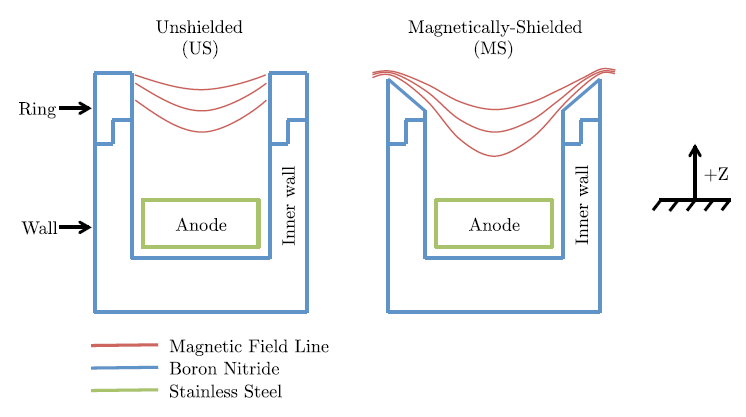
\includegraphics[scale=0.5]{25.png}}
\end{center}

We first need power to the electromagnets that create the magnetic field (couple mps of current). We must supply energy to the discharge supply (200-800V, 1-20A). The heater supply is connected to the cathode and is a coil of wire resistively heating the cathode (few amps). 
\begin{itemize}
\item Heater supply: Raise emitter in hollow cathode to thermionic emission temperature
\item Keeper supply:  Ignition and stable cathode operation. Must apply a voltage between keeper electrode and the actual cathode on the inside. (10s-100sV to get started). Once things started, heater and keeper are turned off. 
\item Discharge supply:  connected between anode and cathode common (and also thruster body and magnetic circuit)
\item Magnet supply:  supply current to electromagnets to create magnetic field
 \end{itemize}

Looking at the potential profile, $V_d$ is the voltage supplied by the discharge supply. $V_b$ is the beam voltage, this beam voltage is the energy the ion actually get. Ion does not get full discharge voltage because of the cathode voltage. The cathode voltage is a little bit lower than ground or space potential and thats to get electrons to come out of the cathode (around 10-20volts below ground) (Electrons what to go up to higher potential so cathode must be below to allow that to happen.)
 
Once discharge started, cathode heater is turned off and cathode runs in "self-heating" mode.  Keeper used only during start-up, turned off when thruster started.
 
Difference between cathode potential and beam potential is the "coupling voltage" (aka cathode voltage).  This is the potential required to extract current from the hollow cathode (typically $\sim$10-20 V, or 5-10$\%$ of $V_d$) (the voltage required to get electrons out of the cathode).  Note the cathode potential will typically be a few volts below space ground (or vac chamber ground in ground tests).
 
The whole circuit floats above ground, it will stabilize itself so that the drop between cathode and discharge is around 10-20V.
 
 Looking at these different voltages....
 
The beam voltage is:
  \begin{equation*}
 \begin{aligned}
 V_b = V_d - V_c
 \end{aligned}
 \end{equation*}
 
In lab experiments, the potential between beam and ground is typically small, so:
 
   \begin{equation}
 \begin{aligned}
 V_b \cong V_d - V_{cg}
 \end{aligned}
 \end{equation}
 
where cathode-to-ground voltage is $V_{cg}$. This is an active research question. It is important to know this so that we have an understanding of the coupling voltage in space. The coupling voltage is dependent on space. In ground experiments we have $v_{cg}$ but will this be the same as when we get into space. We'd like to know this because we'd like to predict our beam voltage. Challenge, understanding the voltage is compared to the one in space. We find that the facility will actually impact this, ie test is in giant grounded shell (vacuum chamber) and ambient gas in the chamber. 
 
Average beam ion velocity is then:
  \begin{equation}
 \begin{aligned}
 <V_b> = \sqrt{\frac{2 \, e \, \bar{V}_b}{M}}
 \end{aligned}
 \end{equation}
 where average beam voltage is $\bar{V}_b$

Acceleration of ion from creation as it moves down the potential, a distance of $V_b$. NOT LIKE ION THRUSTERS: we don't know where ions are created in hall thrusters, only a general idea....therefore, ions will not travel the same beam voltage because some will have more energy than others.There is a distribution of ions and so we will consider an average velocity and average potential drop. 
\newpage
 \begin{subequations}
Discharge current is net current through discharge supply, and is the electron and ion current arriving at the anode:
   \begin{equation}
 \begin{aligned}
 I_d = I_{ea} - I_{ia} \qquad \qquad \text{to anode}
 \end{aligned}
 \end{equation} %I_ia is small since ions done want to go to the andoe.

Discharge current can also be written as the current to the cathode:

   \begin{equation}
 \begin{aligned}
 I_d = I_e + I_{ic} \qquad \qquad \text{to cathode}
 \end{aligned}
 \end{equation}%Ions also dont want to go the cathode.
 
So we see that the discharge current is approximately the electron current emitted by the cathode which is the electron current collected by the anode.
 
   \begin{equation}
 \begin{aligned}
 I_d \approx I_e \approx I_{ea}
 \end{aligned}
 \end{equation}
 \end{subequations}
A schematic of the current in the discharge is shown below.
 
  \begin{center}
{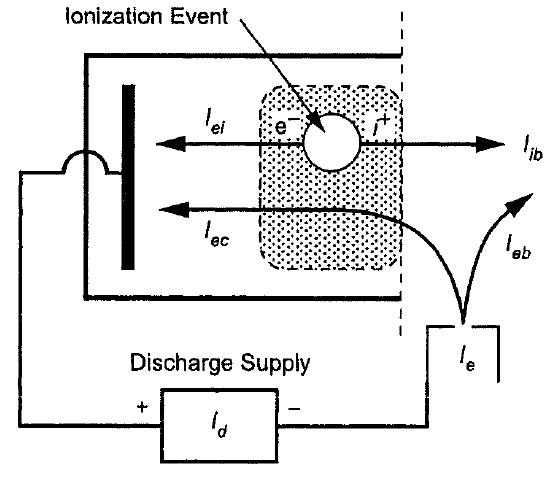
\includegraphics[scale=0.7]{26.png}}
\end{center}
 
 %newpage
 
Current to the anode is electron current emitted by the cathode, and electron current due to secondary electrons from ionization events.  That is:
\newpage
If we look at this figure, the current to this anode is $I_{ec}$ and $I_{ei}$, where $I_{ei}$ is most likely from secondary events while $I_{ec}$ is from primary. 
\begin{subequations}
    \begin{equation}
 \begin{aligned}
 I_d = I_{ec} + I_{ei}
 \end{aligned}
 \end{equation}
 
But as we saw in (9.56c), the discharge current is also essentially the electron current emitted by the cathode, that is:
 
    \begin{equation}
 \begin{aligned}
 I_d \approx I_e = I_{ec} + I_{eb}
 \end{aligned}
 \end{equation}
 
We recognize that one electron and one ion are made in each ionization event, such that        $I_{ei} = I_{ib}$            	and, therefore (9.57a) becomes,
 
    \begin{equation}
 \begin{aligned}
 I_d = I_{ec} + I_{ib}
 \end{aligned}
 \end{equation}

 %The discharge current is the ___ and the ion current going out into the beam. 9.57c is the net current crossing the current plane. 
This is the net current crossing the exit plane, so discharge current is the ion beam current plus the backstreaming electron current crossing the exit plane.
 
 
Finally, comparing (9.57b) and (9.57c), we see:
    \begin{equation}
 \begin{aligned}
 I_{ib} = I_{eb}
 \end{aligned}
 \end{equation}
 
  \end{subequations}
These particles in (9.57d) do not contribute to the discharge current through the discharge supply.  Note in the electrical schematic the entire discharge floats (is not connected to ground).  So there is no return path for these particles to the discharge supply.
 
\subsection{Hall Thruster Performance}
%gamma took into account cosine losses and multiply charged species, we will eave out for now but return to it later. 

Hall thruster total efficiency, like any EP system, is jet power to input electrical power.

     \begin{equation*}
 \begin{aligned}
 \eta_T = \frac{\frac{1}{2} \, T \, I_{SP} \, g_o}{P_{in}}
 \end{aligned}
 \end{equation*}
 
      \begin{equation*}
 \begin{aligned}
T = \dot{m}_i \, v_i \qquad I_{SP} = \frac{T}{\dot{m}_p \, g_o} = \frac{\dot{m}_i \, v_i}{\dot{m}_p \, g_o}
 \end{aligned}
 \end{equation*}
 
 so...
      \begin{equation}
 \begin{aligned}
 \eta_T = \frac{\frac{1}{2} \, T^2}{ \dot{m}_p \, P_{in}}
 \end{aligned}
 \end{equation}
 
 \newpage
Gas flow is split between the anode and cathode.
 
     \begin{equation}
 \begin{aligned}
 \dot{m}_{p} = \dot{m}_{a} + \dot{m}_{c}
 \end{aligned}
 \end{equation}
 
Cathode efficiency is defined as:
 
     \begin{equation}
 \begin{aligned}
 \eta_c = \frac{\dot{m}_{a}}{\dot{m}_{p}}
 \end{aligned}
 \end{equation}
 
where the mass flow rate to the cathode, $\dot{m}_c$            , is lost and does not contribute to thrust/propulsion.
 
 Total power into the thruster is:
 \begin{shaded}
\textbf{Total Power Into Thruster}

     \begin{equation}
 \begin{aligned}
 P_{in} = P_d + P_{mag} + P_k
 \end{aligned}
 \end{equation}
where
\begin{equation*}
\begin{aligned}
P_d &= \text{Discharge power} \\
P_k &= \text{Keeper power (usually zero during thruster operation)} \\
P_{mag} &= \text{Magnet power, power to electromagnets to create Bfield} \\
\end{aligned}
\end{equation*}
\end{shaded}

The electrical utilization efficiency is defined as:
     \begin{equation}
 \begin{aligned}
 \eta_o = \frac{P_d}{P_{\text{total}}} = \frac{P_d}{P_d + P_k + P_{mag}}
 \end{aligned}
 \end{equation}
 
Putting (9.62) and (9.60) into (9.58), yields a useful expression for total HET efficiency:
     \begin{equation}
 \begin{aligned}
 \eta_T = \frac{1}{2} \, \frac{T^2}{\dot{m}_a \, P_d} \, \eta_o \, \eta_c
 \end{aligned}
 \end{equation}
 
Easy to calculate thruster efficiency with (9.63):  measure thrust, know flow split between anode/cathode, know magnet power, keeper power, discharge power.  Plug in, determine efficiency.
 
We can further expand this equation to examine other terms that affect efficiency.  Thrust can be written:
     \begin{equation*}
 \begin{aligned}
 T = \gamma \, \dot{m}_i \, v_i \qquad \qquad \dot{m}_i = \frac{I_b \, M}{e} \qquad \qquad v_i = \sqrt{\frac{2 \, e \, \bar{V}_b}{M}}
 \end{aligned}
 \end{equation*}
 
 such that
 
 \begin{shaded}
 \textbf{Hall Thruster Thrust}
     \begin{equation}
 \begin{aligned}
 T = \gamma \, \sqrt{\frac{2 \, M}{e}} \, I_b \, \sqrt{\bar{V}_b}
 \end{aligned}
 \end{equation}
where
\begin{equation*}
\begin{aligned}
\gamma &= \text{Due to beam divergence (cosine loss), multi-charged species loss} \\
\bar{V}_b &= \text{Average beam voltage, the average potential over which ions are accelerated} \\
&\quad \text{(There is a spread in the beam energy, this is the average value)} \\
I_b &= \text{The beam current} \\
\end{aligned}
\end{equation*}
 \end{shaded}
 
The fraction of discharge current that produces beam current:
 
 \begin{equation}
 \begin{aligned}
 \eta_b = \frac{I_b}{I_d}
 \end{aligned}
 \end{equation}
 
The fraction of discharge voltage that becomes beam voltage:
 
     \begin{equation}
 \begin{aligned}
 \eta_v = \frac{\bar{V_b}}{V_d}
 \end{aligned}
 \end{equation}
 
Put (9.64)(9.65)(9.66) into (9.63) $\rightarrow$
     \begin{equation}
 \begin{aligned}
 \eta_T = \gamma^2 \, \frac{M}{e} \, \frac{I_d}{\dot{m}_a} \, \eta_b^2 \, \eta_v \, \eta_c \, \eta_o
 \end{aligned}
 \end{equation}
 
 
Finally recognize that (9.30) and (9.65) are:
     \begin{equation}
 \begin{aligned}
 \dot{m}_i = \frac{M}{e} \, I_d \, \eta_b
 \end{aligned}
 \end{equation}
 
and
     \begin{equation}
 \begin{aligned}
 \eta_m = \frac{\dot{m}_i}{\dot{m}_p}
 \end{aligned}
 \end{equation}
 \begin{shaded}
 \textbf{Total Efficiency}
     \begin{equation}
 \begin{aligned}
  \eta_T = \gamma^2 \, \eta_b \, \eta_v \, \eta_m \, \eta_o
 \end{aligned}
 \end{equation}
where
\begin{equation*}
\begin{aligned}
\gamma &= \text{Losses due to divergence and multi-charged species} \\
\eta_b &= \text{Current utilization efficiency} \\
\eta_v &= \text{Voltage utilization efficiency} \\
\eta_m &= \text{Mass utilization efficiency} \\
\eta_o &= \text{Electrical utilization efficiency} \\
\end{aligned}
\end{equation*}
\end{shaded}
 
HET efficiency is sometimes (often) expressed in terms of the "anode efficiency", which is defined as:
     \begin{equation}
 \begin{aligned}
 \eta_a = \frac{1}{2} \, \frac{T^2}{\dot{m}_a \, P_d} = \frac{\eta_T}{\eta_o \, \eta_c}
 \end{aligned}
 \end{equation}
 
which neglects the losses associated with powering the magnets and keeper, and losses associated with propellant flow to the cathode.
 
Data for these different efficiencies is shown below in the figure for the NASA 173Mv2 HET.
Charge efficiency is losses due to the multiply-charged ion content in the plume.  Anode efficiency is the combination of these four efficiencies.
 
 \begin{center}
{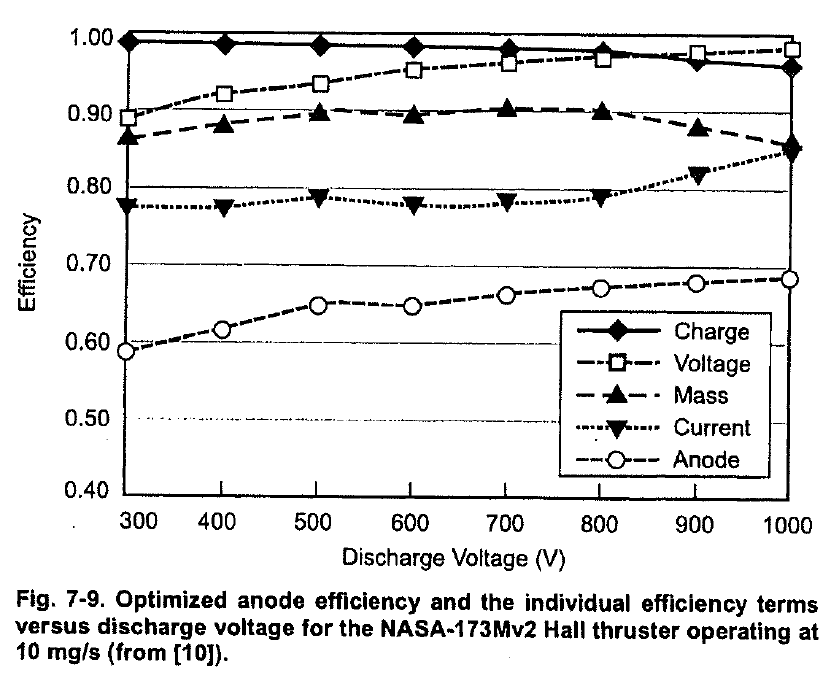
\includegraphics[scale=0.7]{28.png}}
\end{center}
\newpage
\begin{framed}
Why is there a charge utilization efficiency? Why is it inefficiency to use your energy to accelerate doubly charged particles.
     \begin{equation*}
 \begin{aligned}
E = 2eV_b = eV_b + eV_b
 \end{aligned}
 \end{equation*}

Energy we put in to accelerate one double charged particle or two single charged particles. 

\textbf{Double Charged Ion} \\
     \begin{equation*}
 \begin{aligned}
v^{_{+}^{+}} = \sqrt{\frac{4eV_b}{M}} \quad \rightarrow \quad T = Mv^{_{+}^{+}} \sqrt{\frac{eV_b}{M}} \quad \rightarrow \quad \frac{T}{2eV_b} \bigg|^{++} = \sqrt{\frac{M}{e V_b}}
 \end{aligned}
 \end{equation*}
\textbf{Two Single Charged Ion} \\
     \begin{equation*}
 \begin{aligned}
v^{+} = \sqrt{\frac{2eV_b}{M}} \quad \rightarrow \quad T = 2Mv^{+} \quad \rightarrow \quad \frac{T}{2eV_b} \bigg|^{+} = \sqrt{2} \, \sqrt{\frac{M}{e V_b}}
 \end{aligned}
 \end{equation*}
 
 Comparing we get...
      \begin{equation*}
 \begin{aligned}
\frac{T^+}{T^{++}} = \sqrt{2} \quad \rightarrow \quad T^+ \sim 40 \% \text{larger}
 \end{aligned}
 \end{equation*}
 
The thrust we are getting out is about 40$\%$ larger for the singly charged case. 

     \begin{equation*}
 \begin{aligned}
\eta_m^{_{+}^{+}} = \alpha_m \frac{\dot{m}_i}{\dot{m}_p} = \alpha_m \, \eta_m \quad \text{where} \quad \alpha_m = \frac{I^+ + \frac{1}{\sqrt{2}} I^{++}}{I^+ + I^{++}} = \frac{1 + \frac{1}{\sqrt{2}} \, \frac{I^{++}}{I^+} }{1 + \frac{I^{++}}{I^+}}
 \end{aligned}
 \end{equation*}
 
Hall thrusters 10-15$\%$ of the charge is doubly charged.
\end{framed}

\subsection{Power Loss Mechanisms}

In HET power loss to the wall is dominant loss mechanism.  That is, ion and electrons leaving the plasma and going to the wall is dominant loss. The wall material is a dielectric which has a high secondary electron emission rate.

The current deposition and power lost to the walls can be estimated from the sheath potentials and electric fields in the plasma edge, near the wall.  Remember, the wall is an insulator (no conductor), so ion and electron current to the wall must be equal. 
 
However, when an electron bombards the wall, it can cause the wall to emit a "secondary electron".  High-energy electron goes into wall, low energy "secondary" electron may come out of wall.  This secondary electron emission is very important in HET.
 \newpage
Requirement of local net current equal to zero means:
\begin{framed}

 \begin{equation}
 \begin{aligned}
 I_{iw} = I_{ew} - \gamma \, I_{ew}
 \end{aligned}
 \end{equation} 
where
\begin{equation*}
\begin{aligned}
I_{iw} &= \text{Ion current to wall} \\ 
I_{ew} &= \text{Electron current to wall} \\ 
\gamma &= \text{Secondary electron emission coefficient} \\  & \qquad \text{($\#$ secondarys per $\#$ of primaries, non-dimensional, but can be greater than 1 !)}
\end{aligned}
\end{equation*}
 \end{framed}
 
This SEE emission coefficient is measured for different insulator materials common in HET.

 \begin{center}
{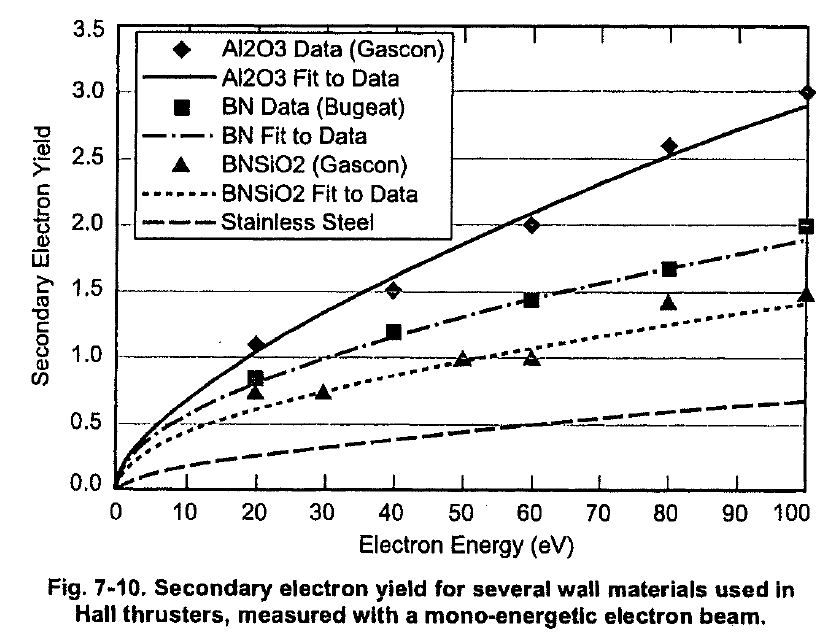
\includegraphics[scale=0.6]{29.png}}
\end{center}
The x-axis is the energy of the electrons hitting the wall. The y-axis is the secondary electron emission yield, the number of electrons coming off the wall from collisions. We want this at a minimum because secondary electron emissions replace high energy, fast moving electrons with slow moving secondary electrons. 

While SEE yield is measured as a function of incident electron energy (eV), we have a population of electrons in Hall thruster with a distribution in energy.  We will assume Maxwellian electron distribution, then SEE yield needs to be integrated over Maxwellian distribution, resulting in: %Integrating the above data we get secondary electrons as a dunction of 
 
  \begin{center}
{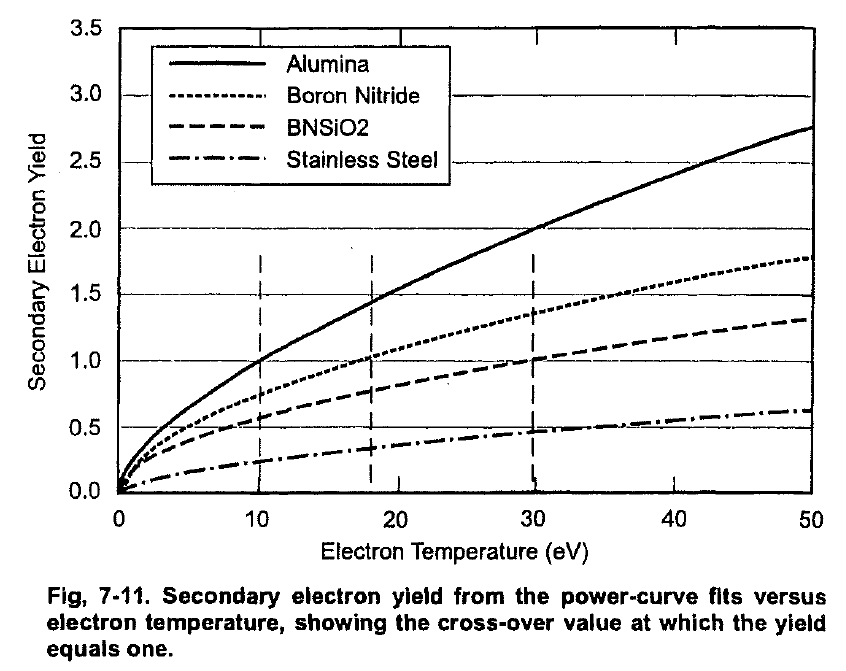
\includegraphics[scale=0.6]{30.png}}
\end{center}
When...

Secondary electrons yield less than one: Not every electrons results in a secondary electrons 

Secondary electron yield greater than one: Every electron results in another electron coming off
 
There is a sheath (boundary) between the plasma and the insulator wall.  Ion current leaving the plasma, entering the sheath, and going to the wall is the Bohm current (used also in (9.3)).  Electron current leaving the plasma, entering the sheath, and going to the wall is (9.15).  Also, assume secondary electrons have no velocity coming off the wall.  Put (9.3) and (9.15) into (9.72),  to get the sheath potential at the wall:
 
  \begin{equation*}
 \begin{aligned}
 I_{iw} &= \frac{1}{2} \, n_i \, e \, A \, \sqrt{\frac{k \, T_e}{M}} \\ \\
 I_{ew} &= \frac{1}{4} \, \sqrt{\frac{8 \, k \, T_e}{\pi \, m}}\, n_e \, e \, A \, \exp \bigg(\frac{e \, \phi}{k \, T_e}\bigg)
 \end{aligned}
 \end{equation*}
 
 
  \begin{equation}
 \begin{aligned}
 \phi_s = -\frac{k \, T_e}{e} \, \ln \bigg[(1-\gamma)\sqrt{\frac{2 \, M}{\pi \, m}}\bigg]
 \end{aligned}
 \end{equation}
 \newpage
This is the sheath potential, the potential drop they will see from the plasma to the wall. It is important to notice how this equation changes based on gamma, the secondary emission yield. If gamma is less than 1, everything inside the logarithm is positive but if gamma is greater, now we cant take the logarithm anymore. Now we have to consider what happens as gamma approaches 1. We see that out sheath potential potential flips from negative to positive. 
 
We see that the sheath potential will go to zero and flip sign (changes from negative-going to positive-going sheath) as the SEE yield goes to 1.
 
 \begin{center}
 \vspace{60mm}
 \textbf{Figure: Sheath Potential Profile}
 \end{center}
 
But actually what limits this secondary electron emission from the wall is NOT the SEE yield, it is the space-charge limit.  Sheath is space-charge limited.  The current of electrons that can come off wall is limited by space-charge, not SEE coefficient.

As secondary electron emission increases, why does space-charge limit become a thing? The potential wont rise as dramatically, no! There is a limit in the current we can pull of the wall from the sheath.

 \begin{center}
 \vspace{60mm}
 \textbf{Figure: Space Charge Limit}
 \end{center}

The more electrons that pop off, we develop a cloud of electrons. The cloud of electrons make it harder for future electrons to come off.  To get even more electrons, I must decrease the gap length or increase the voltage. The sheath will never actually flip as we predicted, the space charge limit effects prevent this...
 
Hobbs and Wesson (1967) studied space-charge limited sheaths with secondary electron emission.  Their results for xenon show that the space-charge limited sheath potential is:
 
 \begin{shaded}
 \textbf{Space-Charge Limited Sheath Potential}
 
   \begin{equation}
 \begin{aligned}
 \phi_o = -1.02 \, \frac{k \, T_e}{e}
 \end{aligned}
 \end{equation}
 \end{shaded}
 
and the corresponding SEE coefficient for the sheath to be space-charge limited is:
 
   \begin{equation}
 \begin{aligned}
 \gamma_o = 1 - 8.3 \, \bigg(\frac{m}{M}\bigg)^{\frac{1}{2}} = 0.983 \text{ for Xe}
 \end{aligned}
 \end{equation} 
 As the potential is changing, it will never go past 0.983 because of the space charge limit. 
 
We see from the Figures above, for typical insulators and HET electron temperatures (>20eV), the SEE coefficient is >1 and is space-charge limited. So for typical HET operating parameters $T_e>20ev $, the sheath at the insulator wall is space-charge limited with a potential drop given by Equation 9.74
 
So, without SEE, the sheath potential would be
 
   \begin{equation*}
 \begin{aligned}
 \phi_{sheath} (\text{No SEE,} \gamma=0) = -5.97 \, T_{e_{[eV]}}
 \end{aligned}
 \end{equation*}
 
But as the SEE coefficient increases, the sheath potential transitions from being governed by SEE to being governed by space-charge, and the sheath potential is:
 
   \begin{equation}
 \begin{aligned}
  \phi_{sheath} = -1.02  \, T_{e_{[eV]}}
 \end{aligned}
 \end{equation}
 
 In between these two extremes (SEE = 0 to SCL sheath) there is strong dependence on electron temperature and the specific channel material, per Eqn. (9.73).
 
Total power to the wall is then the energy carried out by ions and the energy carried out by electrons:
   \begin{equation}
 \begin{aligned}
 P_w = \frac{1}{4} \,\sqrt{\frac{8 \, k \, T_e}{\pi \, m}}\, e \, n_o \, A \,  \exp \bigg(\frac{e \, \phi_s}{k \, T_e}\bigg) \, \bigg(2 \, \frac{k \, T_e}{e}\bigg) + n_o \, V_o \, e \, A \, (\varepsilon - \phi_s)
 \end{aligned}
 \end{equation}
 
 
which can be rewritten:

 \begin{shaded}
 \textbf{Total Power to the Wall}
   \begin{equation}
 \begin{aligned}
 P_w = I_{iw} \Bigg[\bigg(\frac{M}{2 \, \pi \, m}\bigg)^{\frac{1}{2}} \exp \bigg(\frac{e \, \phi_s}{k \, T_e}\bigg) \, \bigg(\frac{2 \, k \, T_e}{e}\bigg) + (\varepsilon - \phi_s)\Bigg]
 \end{aligned}
 \end{equation}
 
where
   \begin{equation*}
 \begin{aligned}
n_o &= \text{Plasma density at sheath edge ($\sim 1/2$ the total plasma density)} \\
\phi_s &= \text{The sheath potential, given by (9.76) or (9.73) depending on $T_e$} \\
&\qquad \text{and corresponding SEE  coefficient.} \\
\varepsilon = 0.58 \, T_e &: \text{Ion KE entering the sheath and is approximately the Bohm energy of $\sim 0.5 T_e$} \\
 \end{aligned}
 \end{equation*}
\end{shaded}



\end{document}